
\documentclass{jsarticle}

\usepackage[dvipdfmx]{hyperref,graphicx,color}
\usepackage{pxjahyper}
\usepackage{ascmac}
\usepackage{listings,jlisting}

\definecolor{mygreen}{rgb}{0,0.6,0}
\lstset{
  basicstyle={\ttfamily},
  identifierstyle={\small},
% commentstyle={\smallitshape},
% keywordstyle={\small\bfseries},
% stringstyle={\small\ttfamily},
  commentstyle=\color{mygreen}\textit,
  keywordstyle=\color{blue}\bfseries,
  stringstyle=\color{red},
  ndkeywordstyle={\small},
  frame=single,
  breaklines=true,
  columns=[l]{fullflexible},
  tabsize=4,
  numbers=left,
  xrightmargin=0zw,
  xleftmargin=0zw,
  numberstyle={\scriptsize},
  lineskip=-0.5ex
}
\lstdefinelanguage{VBA}{
 morekeywords={Private,Set,Call,MsgBox,End,Function,ReDim,If,Return,
	Else,Then,For,Next,To,With,New,As,Sub,Double,Sqr,CVErr,Trim,Str,Me,True,
	False,Int},
 morestring = [d][\color{red}]{"},
 morecomment=[l][\color{mygreen}\textit]{'}
}

\renewcommand{\familydefault}{\ttdefault}

\begin{document}

\begin{center}
 \texttt{\LARGE VBA と Python の比較\\
	― QuadFncクラスの実装を例に ―}
\end{center}

\smallskip

\section*{VBA の場合}

\begin{lstlisting}[language=VBA,title=CommandButton1をクリックした時のプロシージャ]
Private Sub CommandButton1_Click()
    Set myFnc = New QuadFnc
    Call myFnc.init(2, 3, -4)
    Call myFnc.solve(sols)
    msg = "solutions of " & myFnc.str_() & "=0 :" & vbCrLf
    msg = msg & "(" & Str(sols(0)) & "," & Str(sols(1)) & ")"
    MsgBox msg
    Call myFnc.plot(-3, 1, 0.1)
End Sub
\end{lstlisting}

\lstinputlisting
	[firstline=11,language=VBA,title=QuadFnc.cls(使用する workbook の VBAProject に追加)]
	{QuadFnc.cls}
\hfill 2,242 bytes

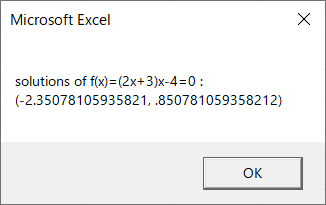
\includegraphics[width=5cm]{img/msgBox.png}\quad
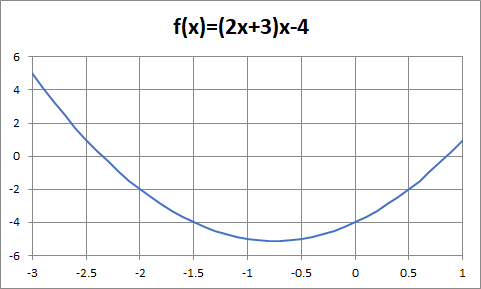
\includegraphics[width=8cm]{img/fig_xls.png}

\section*{Python の場合}

\lstinputlisting
	[language=Python,title=quadFnc.py,morekeywords={int,pow,as,__name__,__str__,self,__init__}]
	{quadFnc.py}
\hfill 899 bytes

\noindent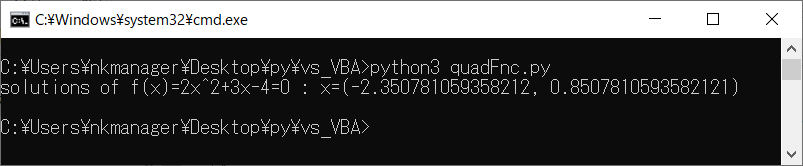
\includegraphics[width=12cm]{img/cmd.png}\\
\noindent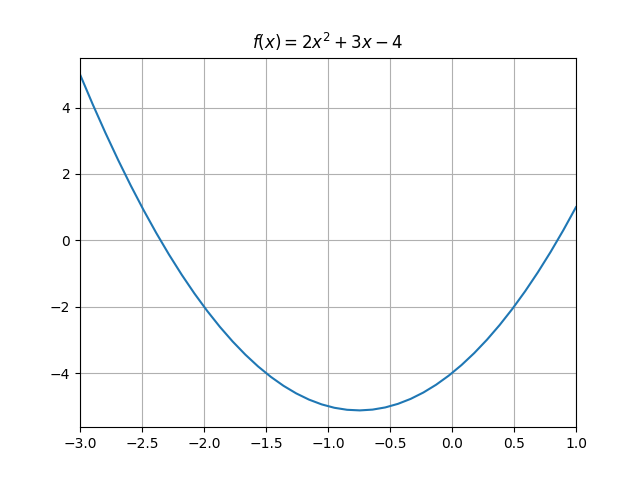
\includegraphics[width=8cm]{img/fig_py.png}

この QuadFnc クラスは以下のように記述することで他のプログラムで容易に利用することができる
\footnote{useCls.py の実行時に quadFnc.py の 34 行目以降は無視される(33 行目が否)。}。

\lstinputlisting
	[language=Python,title=useCls.py]
	{other.py}

\end{document}
